\section{Using cloud computing}
\label{sec:cloudcomputing}

Throughout this book, we assumed that all tasks can actually be
performed on your own computer. And often, that is indeed the best
thing to do: you often want to maintain a local copy of your data
anyway, and it may be the safest bet for ethical and legal reasons --
when working with sensitive data, you need to know what you are doing
before transferring them somewhere else.

However, once you scale up your project, problems may arise (see \cite{Trilling2018b}):
\begin{itemize}
\item Multiple people need to work on the same data
\item Your dataset is too large to fit on your disk
\item You do not have enough RAM or processing power
\item Running a process simply takes too long (e.g., training a model
  for several days) or needs to be run in continous intervals (e.g.,
  scraping news articles once an hour) and you need your computer for
  other things.
\end{itemize}

This is the point where you need to start moving your project to some
remote server instead. Broadly speaking, we can consider three
scenarios:
\begin{enumerate}
\item A cloud service that just lets you run code. Here, you can just
  submit your code and have it run. You do not have full control, you
  cannot set up your own system, but you also do not have to do any
  administration.
\item A dedicated server. You (or your university) could buy a
  dedicated, physical server to run computational social science
  analyses. On the bright side, this gives you full control, but it is
  also not very flexible: after all, you make a larger investment
  once, and if it turns out that you need more (or less) resources,
  then it's too late.
\item A virtual machine on a cloud computing platform. For most
  practical purposes, you can do the same as in the previous option,
  with a crucial difference that you rent the resources. If you need
  more, you just rent more; and when you are done, you just stop the
  machine.
\item A set of machines to run complex tasks using parallel computing. With large amounts of information (think about image or video data) and sophisticated modelling (such as deep learning) you may need to distribute the computation among different computers at the same time.
\end{enumerate}

An example for the first option is Google Colab, which we already used
(\refchap{fundata}). While it makes it easy to share and run notebooks,
the free tier we used so far does not necessarily solve any of the
scalability issues discussed. However, Google Colab also has a paid Pro
version, in which additional hardware (such as GPUs, TPUs or extra memory)
that you may not have on your own computer can be used. This makes
it an attractive solution for enabling projects (e.g., involving
resource-intensive neural networks) that otherwise would not be possible.

However, this is often not enough. For instance, you may want to run
a database (\refsec{databases}) or define a so-called \pkg{cron} job,
which runs a specific script (e.g., a web scraper) at defined intervals.
Here, options 2 and 3 come into play -- most realistically for most
beginners, option 3.

There are different providers for setting up VMs in the cloud, the
most well-known probably being Amazon Web Services (AWS) and
Microsoft Azure. Some universities or (national) research infrastructure
providers provide high-performance computing in the cloud as well.
While the specific way of how to set up an own virtual machine on
such an infrastructure varies, the processes are roughly similar:
You select the technical specifications such as the number of CPU
cores and the amount of memory you need, attach some storage, and
select a disk image with an operating system, virtually always some
Linux distribution (Figure~\ref{fig:createvm}).
After a couple of minutes, your machine is ready to use.

\begin{figure}[!tbp]
  \centering
  \begin{minipage}[b]{0.45\textwidth}
    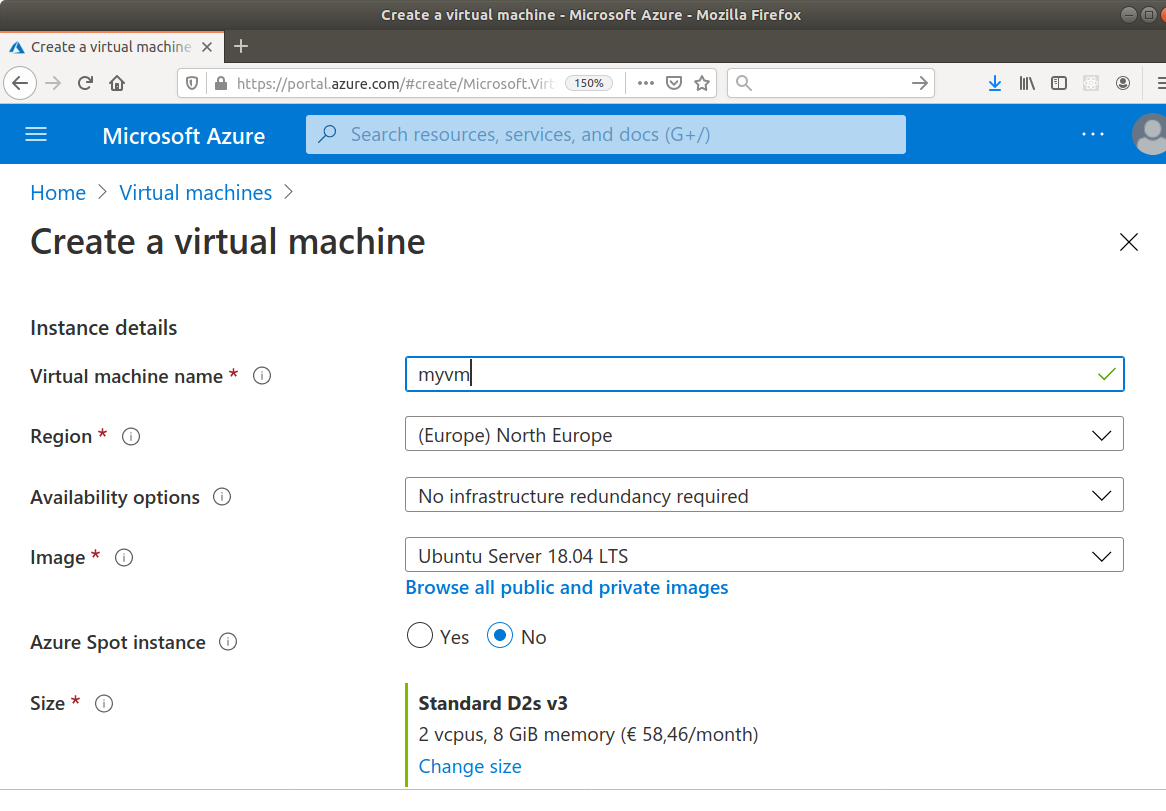
\includegraphics[width=\textwidth]{figures/vmazure.png}
    %\caption{Creating a VM on Microsoft Azure}
  \end{minipage}
  \hfill
  \begin{minipage}[b]{0.45\textwidth}
    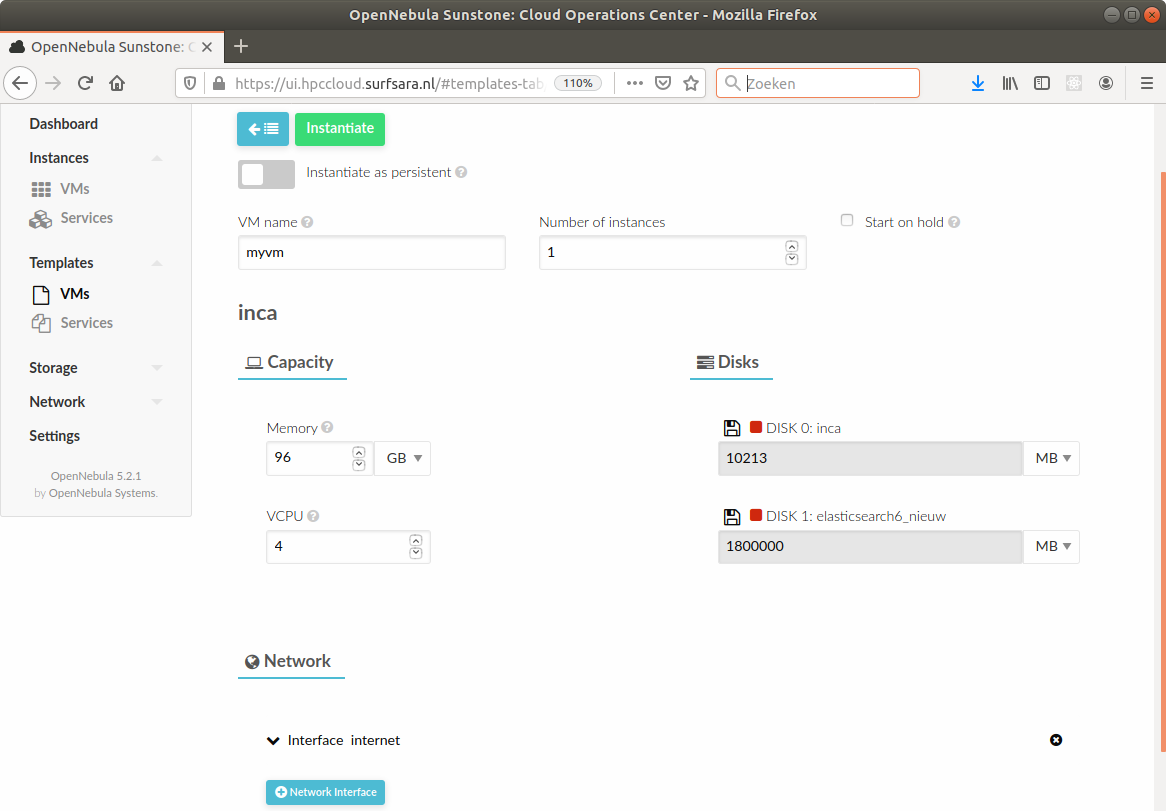
\includegraphics[width=\textwidth]{figures/vmopennebula.png}
    %\caption{}
  \end{minipage}
  \caption{Creating a Virtual Machine on Microsoft Azure (left) and on a university cloud computing platform using OpenNebula (right).\label{fig:createvm}}
\end{figure}

While setting up such a machine is easy, some knowledge is required
for the responsible and safe administration of the machine, in
particular to prevent unauthorized access.

Imagine you have a script |myscript.py| that takes a couple of days to
run. You can then use the tool |scp| to copy it to your new virtual
machine, log on to your virtual machine using |ssh|, and then -- now
on your virtual machine! -- run the script using a tool such as
|nohup| or |screen| that will start your script and will keep running
it (Figure~\ref{fig:ssh}). You can safely logout again, and your
virtual machine in the cloud will keep on doing its work. The only
thing you need to do is collect your results once your script is done,
even if that's a couple of weeks later. Or you may want to add your
script to the crontab (google it!), which will automatically run
it at set intervals.

\begin{figure}[!tbp]
  \centering
  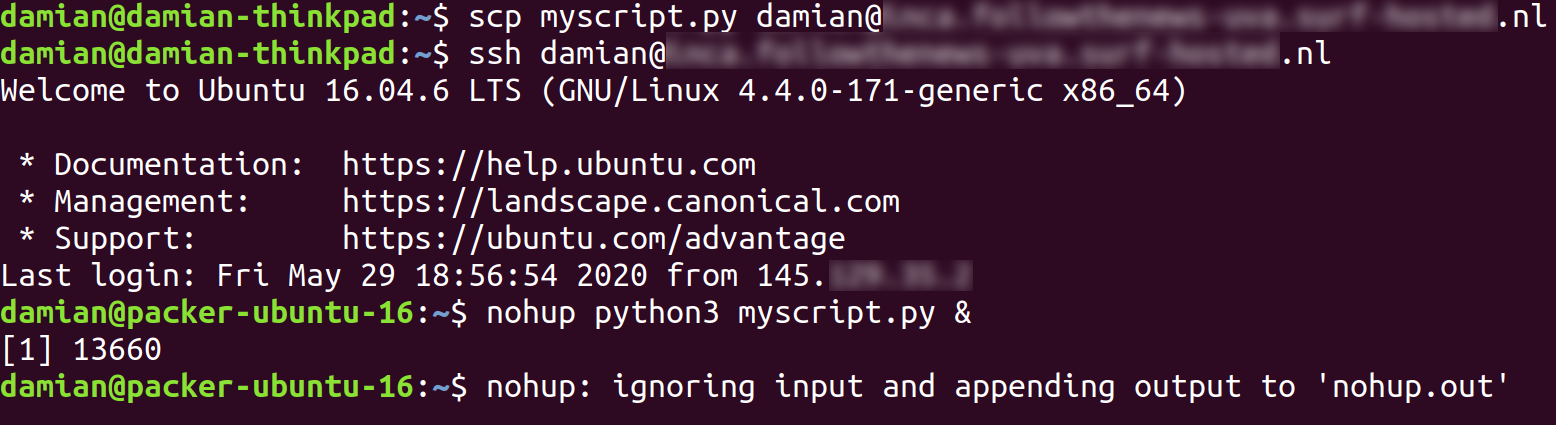
\includegraphics[width=\textwidth]{figures/ssh.png}
  \caption{Running a script on a virtual machine\label{fig:ssh}. Note that the first two commands are issued on the local machine (``damian-thinkpad'') and the next command on the remote machine (``packer-ubuntu-16'')}
\end{figure}

You may want to have some extra luxury, though. Popular things to
set up are databases (\refsec{databases}) and \pkg{JupyterHub}, which
allows users such as your colleagues to connect through their
web browser with your server and run their own Jupyter Notebooks
on the machine. Do not forget to properly encrypt all connections,
for instance using \pkg{letsencrypt}.

Finally, option 4 must be selected when the scale of your data and the complexity of the tasks can not be deployed in a single server or virtual machine. For example, building a classification model by training a complex and deep convolutional neural network with millions of images and update this model constantly may require the use of different computers at the same time. Actually, in modern computers with multiple cores or processors you normally run paralleling computing within a single machine. But when working at scale you will probably need to set a infrastructure of different computers such as that of a \textit{grid} or a \textit{cluster}. 

Cloud services (e.g. AWS, Microsoft Azure, etc.) or scientific infrastructures (e.g. Supercomputers) offer the possibility to set these architectures remotely. For instance, in a computer cluster you can configure a group of virtual computers, where one will act as a \textit{master} and the others as \textit{slaves}. With this logic the master can distribute the storage and analysis of data among the slaves and then resume the results: see for example the \textit{MapReduce} or the \textit{Resilient Distributed Dataset} (RDD) approaches used by the open-source softwares \textit{Apache Hadoop} and \textit{Apache Spark} respectively. 

These architectures for parallel processing will significantly increase your computation capacity for big data problems but the initial implementation will consume time and (most of the time) money, which is the reason why you must think in advance if there is a simpler solution (such as single but powerful single machine) before implementing a more complex infrastructure in your analysis.